 \documentclass[12pt,english]{article}
\usepackage[utf8]{inputenc}
\markright{Pearse et al.\hfill Assessing the Effects Imputation on ED Values\hfill}
\usepackage{geometry}
\geometry{verbose,letterpaper,tmargin=2.54cm,bmargin=2.54cm,lmargin=2.54cm,rmargin=2.54cm}
%\geometry{verbose,letterpaper,tmargin=.1cm,bmargin=.1cm,lmargin=.1cm,rmargin=.1cm}
\usepackage{graphicx}
\DeclareGraphicsExtensions{.pdf,.png,.jpg}
\usepackage{amssymb,amsmath}
\usepackage{epstopdf}
\usepackage{tocbibind}
\usepackage[toc,page]{appendix}
\usepackage{supertabular}
\DeclareGraphicsRule{.tif}{png}{.png}{`convert #1 `dirname #1`/`basename #1 .tif`.png}
\usepackage{url}
\usepackage{subcaption}
\usepackage{caption}
\usepackage[super]{nth}
\usepackage{lineno} \linenumbers
\usepackage[doublespacing]{setspace}
\usepackage[parfill]{parskip}
\setlength{\parindent}{0pt}
\usepackage[citestyle=authoryear,bibstyle=authoryear,sorting=nyt,maxcitenames=2,maxbibnames=10,minbibnames=6,doi=false,url=false,isbn=false,firstinits=true,uniquename=false,uniquelist=false]{biblatex}
\bibliography{edge_sims}
\renewbibmacro*{name:andothers}{% Based on name:andothers from biblatex.def
  \ifboolexpr{
    test {\ifnumequal{\value{listcount}}{\value{liststop}}}
    and
    test \ifmorenames
  }
    {\ifnumgreater{\value{liststop}}{1}
       {\finalandcomma}
       {}%
     \andothersdelim\bibstring[]{andothers}}
    {}}
\renewcommand*{\finalnamedelim}{%
  \ifnumgreater{\value{liststop}}{2}{\finalandcomma}{}%
  \addspace\&\space}
\renewbibmacro{in:}{}
\AtEveryBibitem{%
  \clearfield{day}%
  \clearfield{month}%
  \clearfield{endday}%
  \clearfield{endmonth}%
}
\DeclareFieldFormat[article]{citetitle}{#1}
\DeclareFieldFormat[article]{title}{#1}
\DeclareFieldFormat[article]{pages}{#1}
\DeclareNameAlias{sortname}{last-first}

\usepackage{changes}
\setdeletedmarkup{\textcolor{red}{\sout{#1}}}

\begin{document}
\setlength{\parindent}{0pt}
\section*{Title page}

\textbf{Article title}: Assessing the Effects Imputation on ED Values

\textbf{Running head}: Assessing the Effects Imputation on ED Values

\textbf{Authors:} K.\ Bodie Weedop$^{1}$, William D.\ Pearse$^{1}$\

$^1$ Department of Biology \& Ecology Center, Utah State University,
5305 Old Main Hill, Logan UT, 84322

$^*$To whom correspondence should be addressed:
\url{will.pearse@usu.edu}

\textbf{Word-count}: 5680 (abstract, main text, acknowledgments, and
  references)

\clearpage
\section*{Abstract}

Global extinction rates have been increasing steadily over the recent past
causing a much needed, increased focus on conservation. Conservation triage
provides a decision making criteria to be effective and efficient in setting
conservation priorities. EDGE, an implementation of conservation triage, has
provided a successful foundation and has been applied to set conservation
priorities for a number of taxa (\emph{e.g.} mammals, birds, corals, and
sharks). However, uncertainty has been an issue in each application of EDGE and
remains an issue today. Phylogenetic uncertainty is one source of uncertainty
yet to be properly addressed. The goal of this study was to investigate and
model the effect phylogenetic uncertainty (\emph{e.g.} missing species) and
current methods to compensate for such uncertainty has on EDGE scores. We
evaluate the effect that missing species has on EDGE scores and see that the
removal of missing species has little effect on species remaining in the
phylogeny. Further, we analyze how imputing missing species affects EDGE scores
and whether it is a defensible method of including missing species. We show that
imputation alters the EDGE scores and rankings for species within clades where
imputation is being applied.

\textbf{Keywords}: 

\clearpage
\section*{Introduction}

Evidence from the fossil record and present-day studies argue we are in the
midst of, or entering, a sixth mass extinction \autocite{Barnosky2011,
Ceballos2015}, such that more species than ever are declining and/or in danger
of extinction across a range of environments \autocite{Wake2008,Thomas2004}.
Habitat destruction \autocite{Brooks2002}, invasive species
\autocite{Molnar2008}, climate change \autocite{Pounds2006}, and disease 
\autocite{Lips2006} are some of the leading causes of species declines globally.
Conservation biologists seek to reverse these declines and their detrimental
effects on species populations, but in reality they have limited resources with
which to do so. This challenge, termed the ``Noah's Ark problem''
\autocite{Weitzman1998}, has driven conservation biologists to prioritize, or
triage, the resource allocation \autocite{Bottrill2008}.

Conservation triage, like all sound decision-making, requires some metric that
quantifies the urgency for conservation a set of species. By using such a
metric, researchers are able to avoid biasing the allocation of time and
resources for conservation, and can make their conservation goals more explicit.
One such triage strategies which has been widely used is the EDGE
metric\autocite[Evolutionary Distinction and Globally Endangered;][]{Isaac2007}.
This method prioritizes species according to two criteria: Evolutionary
Distinctiveness (ED) and Global Endangerment (GE). ED measures relative
contributions to phylogenetic diversity made by each species within a particular
clade \autocite{Isaac2007}, assigning each branch length equally to all its
subtending species. GE values are assessed by assigning numerical values to each
of the World Conservation Union (IUCN) Red List Categories. As species become
increasingly threatened and are placed into more concerning categories
(\emph{e.g.}, from Vulnerable to Endangered), the GE numerical value increases.
Thus a species' EDGE score is intended to equally reflect a species'
evolutionary distinctiveness and conservation status \autocite{Pearse2015}.

The EDGE approach was never intended to be a purely academic metric, and is now
the basis of the global EDGE of Existence Program
(\url{http://www.edgeofexistence.org/}). While EDGE was originally used to
prioritize global mammals, it has subsequently been applied to a number of
species groups.

There are now EDGE lists of amphibians \autocite{Isaac2012}, birds 
\autocite{Jetz2014}, corals \autocite{Curnick2015}, and sharks
\autocite{Stein2018}. A number of similar metrics  have been developed, each
prioritizing and emphasizing subtly different things, such as the expected
contribution of each species to overall phylogenetic diversity
\autocite[HEDGE;][]{Steel2007}, our uncertainty over a species' future
\autocite[EDAM;][]{Pearse2015}, and the complementarity of a set of species
\autocite{Faith2008,Jensen2016}. Thus the development of EDGE-like metrics has
matched progress with other fields of conservation biology, where the likelihood
of success in conservation \autocite{Wilson2007, Mcbride2007}, relative cost of
certain interventions\autocite{Naidoo2006}, and complementarity of
interventions \autocite{Pressey1993, Myers2000} have also been considered.
Critically, EDGE has formed the basis of a successful program that
quantitatively prioritizes conservation, providing actionable insights into how
to focus conservation effort in the face of uncertainty about species'
attributes. EDGE's success proves that phylogenetic conservation prioritization
metrics can be used by conservation biologists and policy makers, and that they
are popular with the public. Nonetheless, almost every application of an
EDGE-like approach has had to deal with the uncertainty presented by missing
species data.

IUCN has given guidance that any available contextual data should be used to
assign some threat status to species which are Data Deficient species
\autocite{Iucn2001, Iucn2008}. A number of studies have been done showing how to
follow this guidance and assign threat categories to Data Deficient species and
reduce the uncertainty in GE \autocite{Good2006, Butchart2010, Morais2013}. The
problem, however, is arguably more complex for species whose phylogenetic
position is unknown. Species of conservation concern are almost by definition
rare, and so we frequently lack sufficient DNA (or even morphological) data to
place them with certainty on a phylogeny. In the face of such essentially
unavoidable uncertainty, conservation biologists have worked hard to overcome
data limitations. In most empirical EDGE lists, taxonomic information, rather
than sequence data alone, is used to locate species in the tree of life
\autocite{Isaac2007, Isaac2012, Collen2011, Jetz2014, Curnick2015, Stein2018,
Gumbs2017}. By using taxonomic information alone, researchers are able to
produce fully resolved phylogenies using model-based imputation
\autocite{Kuhn2011, Thomas2013}. Yet, to our knowledge, there has yet to be a
systematic study of the effect of such imputation on species' EDGE scores,
unlike in other aspects of comparative biology \autocite{Rabosky2014}. Indeed,
there is no clear guidance as to the size of the effect of ignoring missing
species on remaining species during prioritization, or the magnitude of error
phylogenetic imputation introduces. As the desire to use ED and phylogenies for
conservation triage grows, the importance of such tests and a consensus on how
to resolve cases of phylogenetic uncertainty becomes more urgent.

Here we quantify the effect of missing species on EDGE rankings and assess
whether imputing species is a defensible method for dealing with species missing
phylogenetic data. We do so by simulating the removal of species from simulated
trees in two ways: at random and in a phylogenetically biased manner. By doing
so, we hope to provide two reasonably realistic case-studies of how species
might be expected to be missing from the tree of life. We also assess the extent
to which imputed species' EDGE rankings correlate with their true values. To do
this, we simulate phylogenies, choose clades at random to remove, and then
impute the structure of these clades, all under the same model of
diversification. In so doing, we hope to provide clear guidance as to the
applicability of phylogenetic imputation as a solution for species missing
phylogenetic data. From our results, we argue that species' ED values are
remarkably robust to the loss of species, and that phylogenetic imputation is
not reliable at reconstructing the true ranking of species.

\section*{Methods}

Here we use a simulation approach to test the effect of removing and imputing
species on a phylogeny on species' ED (Evolutionary Distinctiveness) scores.
Since empirical studies do not (to our knowledge) impute GE (Global
Endangerment) scores for species, instead relying on the IUCN's proposal to
assign Data Deficient species as threatened or otherwise based upon any
available evidence, we focus solely on phylogenetic imputation. EDGE is the
product of both ED and GE, thus perfectly accurate GE values could still lead to
a biased EDGE score if the ED scores were imperfectly calculated.

All simulations and analyses were performed using R \autocite[version
3.4.0;][]{R2017}, and we performed 100 replicate simulations of each parameter
combination . All trees (both starting and imputed) were simulated under a
pure-birth Yule model using the \texttt{sim.bdtree} function under parameters of
\textt{(b=1, d=0)} in the \texttt{geiger} R package \autocite{Pennell2014}. 
This particular model was chosen because it is the simplest model possible:
speciation rates are constant across the entire tree of life and there is no
extinction. We acknowledge that it is possible that more complex and/or
biologically realistic models of diversification could improve the performance
of imputation. However, we suggest that imputation under a simple model that is
identical to that used to simulate the data is a low benchmark for a method to
surpass. We used \texttt{ed.calc} in the R package \texttt{caper} to calculate
ED values \autocite{Orme2013}.

\subsection*{The impact of missing species on EDGE scores}
Our first set of simulations assesses the impact of random and
phylogenetically-biased loss of species from a phylogeny on ED scores. Both sets
of simulations were carried out using phylogenies of different sizes (number of
taxa: 64, 128, 256, ..., 2048, 4096), removing constant fractions of tips from
the tree (0\%, 1\%, 2\%, ..., 19\%, ..., 99\%). To simulate randomly missing
species, we used the \texttt{sample} function in R to select the relevant
percentage of species (rounded to the nearest whole number) without replacement.
Thus this randomization did not incorporate phylogenetic structure. To remove
species in a phylogenetically biased manner, we used
\textcite{Felsenstein2005}'s threshold model. First, we simulated a trait under
a constant rate Brownian-motion model ($\sigma^2$=0.5, starting root value = 1).
using the \texttt{sim.char} function in the \texttt{geiger} R package
\autocite{Pennell2014} Species were then removed from the tree if their
simulated trait was in the upper quantile of whatever fraction of species were
to be dropped. For example, if 10\% of species were to be dropped, species
within the upper \nth{10} quantile of character trait values were removed from
the tree. 

We calculated species' ED values before removal of species from the tree and
afterwards. We then correlated the ED scores (using the \texttt{cor} function in
the \texttt{stats} R package) of the species left in the tree with their
original ED values, to measure the effect of species' removal on ED scores (fig.
\ref{missingSpecies}). If missing species have no effect upon ED values, we
expect a high, positive coefficient of correlation between the remaining
species' ED scores before and after the other species were removed from the
tree.

\begin{figure}[!ht]
  \center
  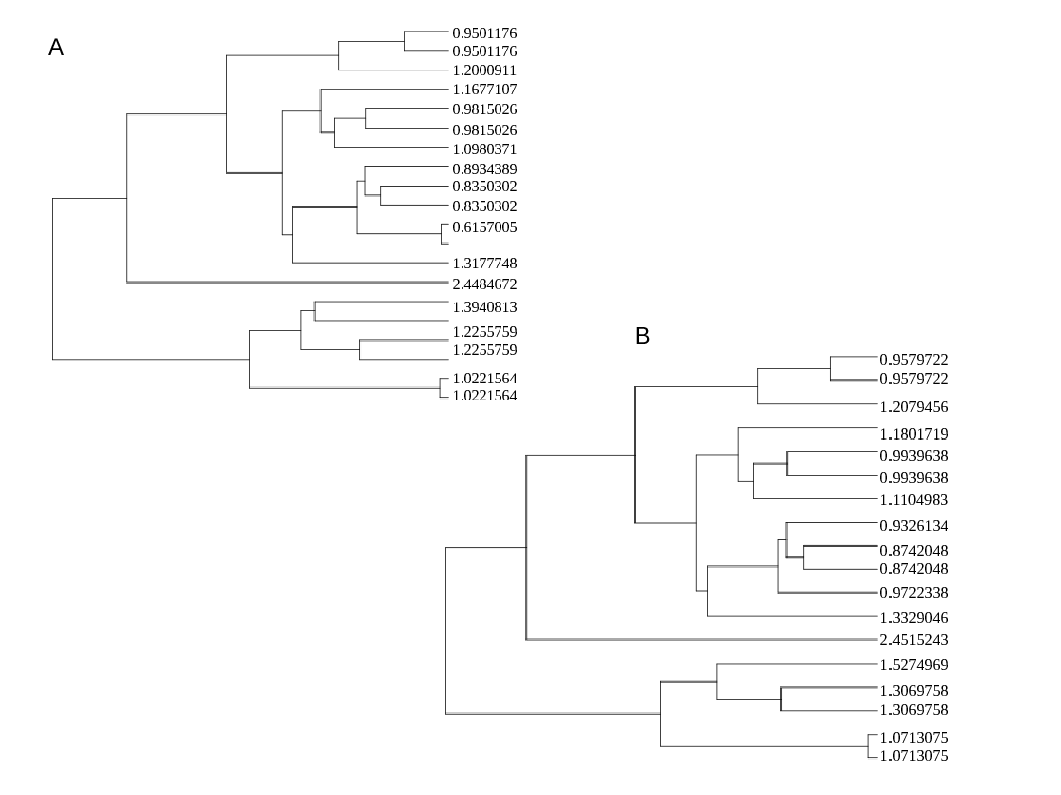
\includegraphics[width=.5\textwidth]{missingSpecies.png}
  \caption{\textbf{Example of simulated phylogenies and ED values used to
  compare species ED values.} The simulated tree on the right (A) is the true
  tree prior to removal of missing species. On the left (B), is the same tree
  after missing species have been removed. Each of the ED values for species can
  be seen to the right of each tip. We correlate the remaining ED values to
  compare the ED values. In this example, one species is missing and been
  removed and the correlation coefficient $r$ = 0.976.}
  \label{missingSpecies}
\end{figure}

\subsection*{The impact of phylogenetic imputation on EDGE scores}
We tested the impact of imputing missing species onto clades of various sizes
(3, 4, 5, ..., 30, 31, 32 species) from phylogenies of different sizes (64, 128,
256, 512, and 1024 species). We first randomly selected a clade to be removed
from the original tree, simulated a new phylogeny of the same size under the
same pure-birth model used to generate the phylogeny, and placed the newly
simulated clade back where the original clade was removed. Thus we imputed each
clade under the model used to generate it: in an empirical study this model
would, itself, have to be inferred but we do not address this additional source
of error here. To see if phylogenetic structure or distribution is ED values
could explain variation in the effect of removal and subsequent imputation, we
also recorded, before species were removed from the tree, lambda (using the
\texttt{yule} function in the R package \texttt{ape} \autocite{Paradis2017}),
overall branch length (by summing the branch lengths given by
\texttt{sim.bdtree}), gamma (using the \texttt{gammatest} function in the R
package \texttt{phytools} \autocite{Revell2017}), colless' index (using the
\texttt{as.treeshape} function in the R package \texttt{apTreeshape}
\autocite{Bortolussi2009}), kurtosis (using the \texttt{moments} function in the
R package \texttt{kurtosis} \autocite{Komsta2015}), and skew (using the
\texttt{skew} function in the R package \texttt{moments} \autocite{Komsta2015}).
In cases where a phylogeny was simulated without a clade of the required size,
that particular simulation was aborted and we moved on to the next simulation in
order to obtain a clade of that size.

To assess whether clades, once imputed, had similar ED scores, we correlated the
imputed ED scores against true ED scores. We also calculated the sum of the
absolute change in ranked ED for each species, which is particularly relevant
for EDGE-listing as it is often the top 100, 200, etc., species on which
conservation actions are targeted. We statistically modeled both these metrics
as a function of the number of total species and number of species within an
imputed clade, since we might expect larger clades and/or larger phylogenies to
be imputed more erroneously.

\section*{Results}
Under both random and phylogenetically-patterned loss, species' ED scores are
less accurate as more species are removed from the tree (Table 1; Fig.
\ref{randomVsClustered}). Correlations between ED values before and after 10\%
and 20\% of species are missing at random are \textasciitilde 0.957 and
\textasciitilde 0.882, respectively. When missing 10\% and 20\% of overall
species in the phylogenetically-biased manner we see the correlation coefficient
is higher at \textasciitilde 0.985 and \textasciitilde 0.938.

\begin{figure}[!ht]
  \center
  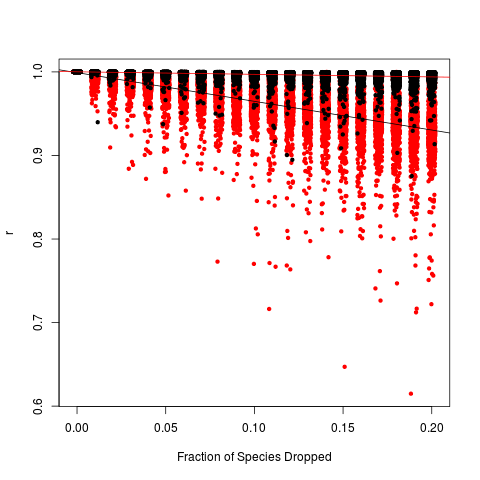
\includegraphics[width=.5\textwidth]{randomVsCluster.png}
  \caption{\textbf{R-values plotted against the fraction of species dropped at
  random versus clustered manner.} The color of data points denote whether
  species were dropped at random (orange; n = 100) or in clustered manner
  (grey; n = 100). The regression lines are demonstrating the relationship when
  species are dropped at random (red) and in a clustered manner (clustered). The
  correlations represent a comparison of the ED values (before and after
  species are dropped) of species which remain on the on the phylogeny after
  other species are dropped. 
  }
  \label{randomVsClustered}
\end{figure}

\begin{table}[ht]
  \centering
  \begin{tabular}{rrrrr}
    \hline
      & Estimate & Std. Error & t value & Pr($>$$|$t$|$) \\
      \hline
      (Intercept) & 1.0315 & 0.0013 & 821.39 & $<$0.0001 \\
      Fraction of Species Dropped & -0.4696 & 0.0020 & -233.16 & $<$0.0001 \\
      Random Treatment & 0.0630 & 0.0018 & 35.47 & $<$0.0001 \\
      Number of Species Overall & 0.0000 & 0.0000 & 7.89 & $<$0.0001 \\
      Fraction of Species Dropped:Random Treatment & -0.2774 & 0.0028 & -97.45 & $<$0.0001 \\
      Random Treatment:Number of Species Overall & 0.0000 & 0.0000 & -4.38 & $<$0.0001 \\
      \hline
    \hline
  \end{tabular}
\caption*{\textbf{Table 1: ANCOVA model summary describing the effect of
dropping species on remaining species ED Values.} The fraction of species
dropped significantly affects the the remaining ED values. Dropping the
fraction both at random and in clustered manner both have negative effects on
the remaining ED values ($F_{139696, 5}$ = 40350, $R^{2}$ = 0.5908,
p$<$0.0001).}
\end{table}

We find no support for a correlation between the imputed and true ED values for
species within imputed clades (Fig. \ref{imputationTrend}, Table 2). We found
that measures of the true phylogeny such as phylogenetic diversity (PD),
estimated rate of diversification $\hat{\lambda}$, Colless' Index, as well as
skew and kurtosis of the distribution ED values do not provide any indication
that imputation would negatively affect ED values (Appendix A). We do find
evidence that, when imputing larger clades, the variation in the correlation is
lesser (Fig. \ref{quantReg}), but the correlation between true and imputed ED
values appear to converge on zero correlation (Table 3). Imputed rankings of
species within clades are also altered under imputation (Fig.
\ref{rankingError}; Table 4). This ranking error increases with the size of the
imputed clade and phylogeny (Table 4), and can affect ranking error within the
top 100, 250, etc. species (Appendix B). For example, within a phylogeny of 1024
species, a species within an imputed clade of 30 species is, on average, \pm 315
rankings from its true ranking.

\begin{figure}[!ht]
  \center
  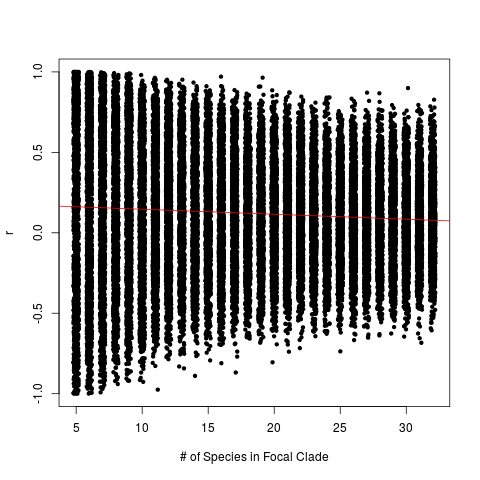
\includegraphics[width=.5\textwidth]{edModel.png}
  \caption{\textbf{R-values plotted against the number of species at focal
  clade.} Each data point denotes a correlative comparison between ED values
  within the focal clades where imputation has occurred. The regression line
  (red) and trend even closer to zero demonstrates the decrease in informative
  value of the imputed ED values. This is reinforced by the visual narrowing of
  r-values around zero.}
  \label{imputationTrend}
\end{figure}

\begin{table}[ht] 
\centering
\begin{tabular}{rrrrr}
  \hline
  & Estimate & Std. Error & t value & Pr($>$$|$t$|$) \\
   \hline
   (Intercept) & 0.1691 & 0.0500 & 3.38 & 0.0007 \\
   Size of Focal Clade & -0.0029 & 0.0002 & -14.15 & 0.0000 \\
   Size of Phylogeny & -0.0001 & 0.0001 & -1.01 & 0.3128 \\
   PD & 0.0001 & 0.0001 & 0.97 & 0.3339 \\
   Lambda & 0.0051 & 0.0492 & 0.10 & 0.9179 \\
   Colless' Index & 0.0020 & 0.0021 & 0.96 & 0.3388 \\
   Skew & 0.0039 & 0.0083 & 0.47 & 0.6409 \\
   Kurtosis & -0.0005 & 0.0008 & -0.64 & 0.5247 \\
   \hline
   \hline
\end{tabular}
\caption*{\textbf{Table 2: Effect of Clade Size on Imputed ED Values.} The
intercept describes that the correlation between the true and imputed values
begins quite low. As the clade size increases, this correlation only tends
toward zero. The total number of species in the full phylogeny along with
measures of the true phylogenetic diversity, lambda, Colless' Index, skew, and
kurtosis show no significant effect. ($F_{47992, 7}$ = 29.38, $R^{2}$ = 0.005,
p$<$0.0001).}
\end{table}

\begin{figure}[!ht]
  \center
  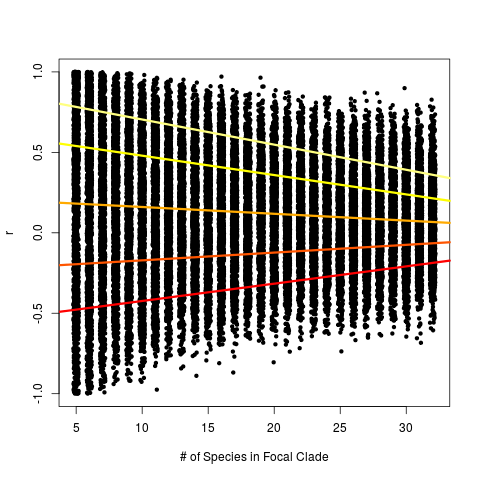
\includegraphics[width=.5\textwidth]{quantModel.png}
  \caption{\textbf{Quantile regression of r-values against size of imputed
  clades.} Each data point denotes a correlative comparison between ED values
  within the focal clades where imputation has occurred. Each regression line
  (top to bottom) represent quantile regressions from highest to lowest,
  respectively. Each of the regression lines demonstrate a convergence of the
  variation in r-values around zero.}
  \label{quantReg}
\end{figure}

\begin{table}[ht]
  \centering
  \begin{tabular}{rrrrrr}
    \hline
  & \tau = 0.10 & \tau = 0.25 & \tau = 0.50 & \tau = 0.75 & \tau = 0.90 \\
    \hline
  (Intercept) & -0.54 & -0.23 & 0.20 & 0.60 & 0.86 \\
    Size of Focal Clade & 0.01 & 0.01 & -0.00 & -0.01 & -0.02 \\
    \hline
    \hline
  \end{tabular}
  \caption*{\textbf{Table 3: Quantile Regression of Clade Size and Total Species
  on Ranking Error.} Quantile regression model demonstrating the effect of clade
  size on the correlation between true and imputed ED values. The quantile
  regression estimates demonstrate statistical significance that as imputed
  clade size increases, variation in coefficient of correlation (r) between ED
  values center around zero (all p-values are $<$0.0001).}
\end{table}


\begin{figure}[!ht]
  \center
  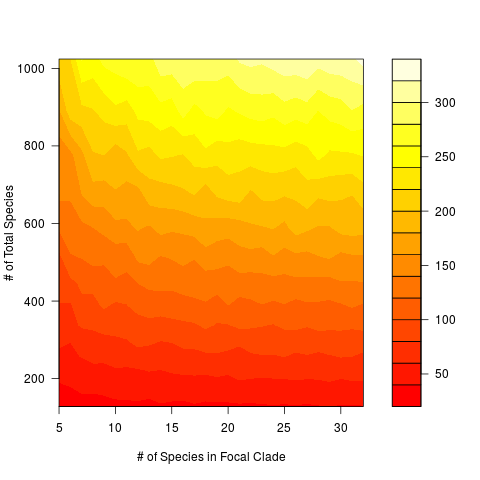
\includegraphics[width=.5\textwidth]{rankingError.png}
  \caption{\textbf{Mean ranking error of species within the focal clade.} The 
  gradient on the right demonstrates average number of positions within the 
  full ranking that focal clade species shifted from their true rank.
  While controlling for the size of the full phylogeny and focal clade, species 
  within the focal clade were, on average, ranked far from the true rank. }
  \label{rankingError}
\end{figure}

\begin{table}[ht]
  \centering
  \begin{tabular}{rrrrr}
    \hline
   & Estimate & Std. Error & t value & Pr($>$$|$t$|$) \\
    \hline
  (Intercept) & -1.6344 & 0.0332 & -49.29 & 0.0001 \\
    Size of Focal Clade & 0.0900 & 0.0010 & 91.22 & 0.0001 \\
    Size of Phylogeny & 0.5179 & 0.0013 & 383.99 & 0.0001 \\
     \hline
     \hline
  \end{tabular}
  \caption*{\textbf{Table 4: Effect of Clade Size and Total Species on Ranking
  Error.} Model demonstrating the relationship between focal clade species
  ranking error and the size of imputed clade and overall phylogeny. Square-root
  transformations have been applied to both ranking error and size of phylogeny.
  Significant increases ranking error are seen when increasing sizes of both the
  imputed clade and phylogeny ($F_{47997, 2}$ = 77890, $R^{2}$ = 0.7644,
  p$<$0.0001).}
  \end{table}

\clearpage
\section*{Discussion}
Phylogeny is increasingly playing a role in conservation prioritization,
decision-making, and policy. A major obstactle to a more widespread adoption of
phylogenetic prioritization methods such as EDGE is phylogenetic uncertainty
\autocite{Collen2015}. We do not have phylogenetic information on all species,
and without this it is difficult to allocate resources to most efficiently
protect the evolutionary history of species. In order to address such
uncertainty, we answered two key questions: (1) the extent to which species that
are missing from the tree of life impact the ED scores of species for which we
do have data, and (2) the extent to which phylogenetic imputation can accurately
fill-in ED scores for taxa with no phylogenetic data. We found that (1) while
missing species do impact the ED scores of other species, the effects are not
always severe and are lesser if species are missing at random from the tre of
life. (2) We found limited evidence that phylogenetic imputation can accurately
reconstruct species' ED scores and rankings.

Our results are derived solely from simulations under a simple model of
diversification---the Yule model. We do acknowledge that, in reality, lineages
evolve in more complex ways than are captured by such a simple model. Yet it is
not obvious to us that these complexities would make imputation easier, and we
suggest that focusing on the simplest model of diversification makes our results
more easily generalizable. Equally, we focus here solely on the results from a
single imputation in each simulation. Normally, pseudo-posterior distributions
of many phylogenies are creates and results reported across averages of these
distributions \autocite{Kuhn2011}. Thus our simulations show that these averages
are conducted across phylogenies with large degrees of uncertainty. It is
well-known that such methods are not biased \autocite[indeed, this was
originally shown by][]{Kuhn2011}: here we emphasize that the uncertainty they
introduce is sufficiently large that they may not be as informative as has
previously been thought.

\subsection*{ED scores are relatively robust to the loss of species}
Missing species and poor phylogenetic resolution have been identified as causes
of uncertainty when calculating ED \autocite{Isaac2007}, but we were unable to
find a quantitative assessment of how missing species might affect ED values of
species which are not missing. Empirically in corals, incomplete phylogenies
produced the same result as later, more complete trees \autocite{Curnick2015}.
Our results support this finding. Our analysis demonstrates that, for example,
missing 20\% of total species, at random and in a phylogenetically-biased
manner, only to a drop in $r$ of 0.882 and 0.938, respectively (Table 1). A drop
in $r$ of only 0.118 and 0.062 between true and imputed ED values is not, in our
opinion, all that concerning when assigning ED scores to remaining species.

We do find that the effect of missing species is more severe when those species
are randomly distributed across the phylogeny. However, perhaps, the most
extreme form could be if an entire clade were missing, and clades that are
geographically restricted to difficult-to-reach regions \autocite[\added{as is
seen with 27 coral species in the Indian Ocean;}][]{Arrigoni2012} are both
difficult to sequence and not uncommon. We have not attempted to comprehensively
simulate all of the different ways in which species could be missing from a
phylogeny. We consider it sufficient to demonstrate that, if species are missing
at random, the effect is not too severe, but that it can be more severe if
missing species are distributed across the phylogeny in a biased fashion. 

\subsection*{Imputation does not reconstruct the ED value of species with great precision}
Our results show that imputation does not accurately recover the true ED values
nor ED rank of missing species (Fig. \ref{imputationTrend}; Fig.
\ref{rankingError}). Thus we argue that, even though under imputation missing
species are incorporated into EDGE lists, their associated EDGE scores may not
reflect their true scores. For example, members of an imputed clade of 25
species within a phylogeny of 850 species are, on average, imputed to have ED
scores 250 ranks away from their true rank (Fig. \ref{imputationTrend}; Table
4).

While we did not assess clades with fewer than five species (we do not consider
correlations or averages to be reliable with so few data-points), we cannot
think why smaller clades would necessarily be more reliable (and this would be a
reversal of the trend in Fig. \ref{imputationTrend}). Indeed, in the smallest
possible clade (two species), imputation is essentially sampling a terminal
branch length from an exponential distribution \autocite{Kuhn2011}; such a
process should still lead to a great degree of uncertainty. It is, perhaps,
unsurprising that imputed ED values do not correlate with their true values (see
table XXX), but we were surprised at the degree of ranking error. Indeed, large
phylogenies showed \emph{greater} ranking error; we na\"{i}vely would have
expected the opposite. We would have expected our upper bound on the age of the
imputed clade, which we would have expected to be relatively younger in larger
phylogenies, to have somewhat controlled the range of the ranks of our imputed
species. ED is known to be driven mostly by terminal branch length
\autocite{Isaac2007,Steel2007}; our results therefore emphasize this.

Imputation is not the only way to incorporate missing species into EDGE-like
frameworks \autocite{Gumbs2017, Collen2011}, but we believe it is the most
common. $3,330$ of birds \autocite[\textasciitilde30\%;][]{Jetz2014}, 250 of
mammals \autocite[\textasciitilde 5.6\%;][]{Collen2011}, and 610 of sharks
\autocite[\textasciitilde49\%;][]{Stein2018} in recent EDGE lists were imputed.
It is well-known that phylogenetic imputation can cause biases in other fields:
\textcite{Rabosky2014} showed that imputation consistently biases evolutionary
rates and estimates of phylogenetic signal \autocite{Rabosky2014}. We emphasize
that we are not, however, suggesting that imputation \emph{biases} ED scores: we
are, instead, suggesting that it is less precise than has previously been
acnkowledged. We discuss, below, the implications of this, and suggest
guidelines for its use.

\subsection*{Guidelines for the use of imputation}
The impact of imputation on EDGE scores is almost certainly lesser than its
impact on ED scores, because EDGE scores are a produce of both ED and IUCN
status. This does not, however, mean that phylogenetic imputation is any less of
a problem. The novelty and purpose of EDGE-like metrics is to incorporate
phylogeny, and if imputed EDGE scores are driven by the GE component because of
the uncertainty introduced by imputation we are accidentally creating a metric
based on IUCN listing alone.

We suggest there is a straightforward synthesis of our results that should be
useful in applied conservation biology. Both random and
phylogenetically-patterned missing species affect ED scores, albeit to differing
extents.  Therefore, conservation biologists should consider using imputation to
mitigate such bias.  We do emphasize, however, that in a phylogeny missing 30\%
of species at random, the mean correlation coefficient ($r$) of the remaining
species' ED scores with their true scores was 0.81 (with variation, of course;
see figure \ref{randomVsClustered}). Where the same proportion of species
missing in a phylogenetically-biased way, the $r$ was 0.891. The problem may not
be as severe as has previously been thought, but that is not reason to try and
mitigate it through imputation.

However, we suggest that prioritizing species whose phylogenetic structure has
been imputed should be done with extreme care. Our simulations show that the ED
rankings, and the top-scored species, are very variable under imputation. If
imputed distributions of trees essentially represent Bayesian posterior
distributions \autocite{Kuhn2011}, then we should treat them as such: the 95\%
posterior densities of these distributions' ED values represent the range within
which we can be 95\% certain the true ED scores lie (if the model assumptions
are met). Our results highlight that the ranges of these distributions are often
much greater than has previously been acknowledged. If we are to avoid
prioritizing the wrong species, we should consider focusing our efforts on those
species whose ED scores we can know with greater certainty: those for which we
have data.

\section*{Acknowledgments}

\clearpage
\printbibliography

\clearpage
\appendix
\section*{A. Effect of Measures of the True, Full Phylogenies}

\begin{figure}[!ht]
  \center
  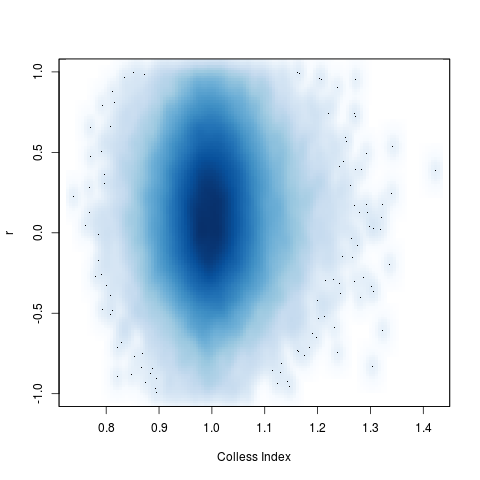
\includegraphics[width=.5\textwidth]{trueColless.png}
  \caption{\textbf{Effect of the True Colless Index of FullPhylogeny.}}
\end{figure}

\begin{figure}[!ht]
  \center
  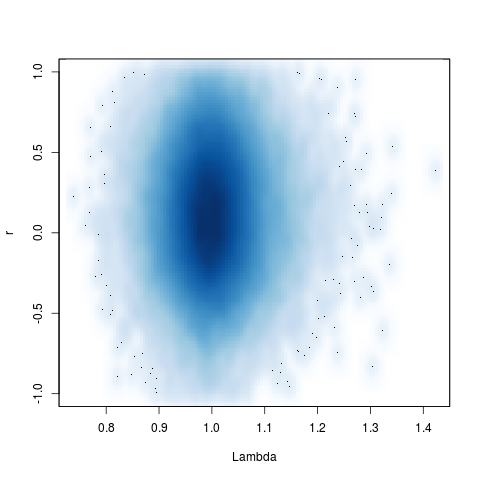
\includegraphics[width=.5\textwidth]{trueLambda.png}
  \caption{\textbf{Effect of the True Lambda of Full Phylogeny.}}
\end{figure}

\begin{figure}[!ht]
  \center
  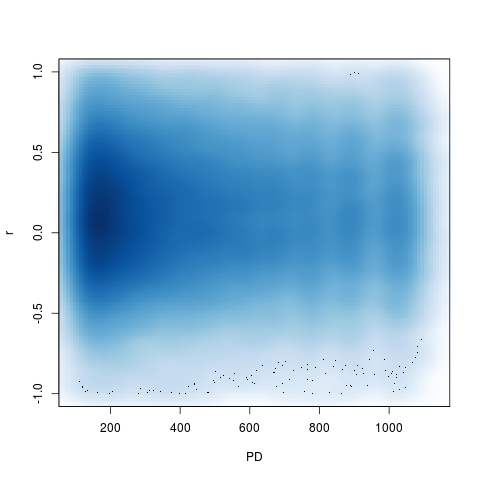
\includegraphics[width=.5\textwidth]{PD.png}
  \caption{\textbf{Effect of True PD of Full Phylogeny.}}
\end{figure}

\begin{figure}[!ht]
  \center
  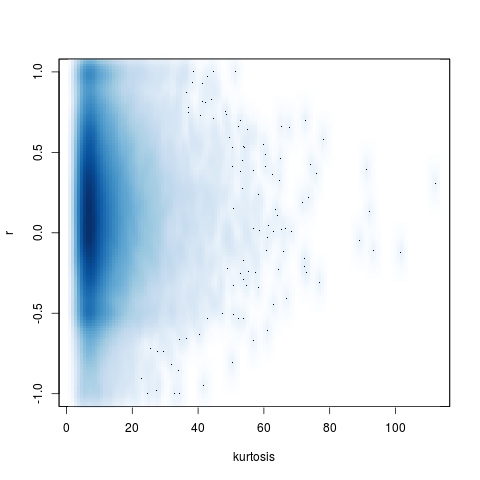
\includegraphics[width=.5\textwidth]{originalKurtosis.png}
  \caption{\textbf{Effect of the True Kurtosis of Full Phylogeny.}}
\end{figure}

\begin{figure}[!ht]
  \center
  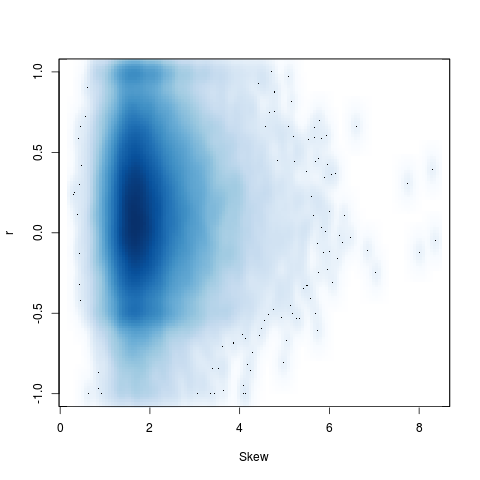
\includegraphics[width=.5\textwidth]{originalSkew.png}
  \caption{\textbf{Effect of the True Skew of Full Phylogeny.}}
\end{figure}

\clearpage
\clearpage
\section*{B. Error Rate in Top Rankings}

\begin{figure}[!ht]
  \center
  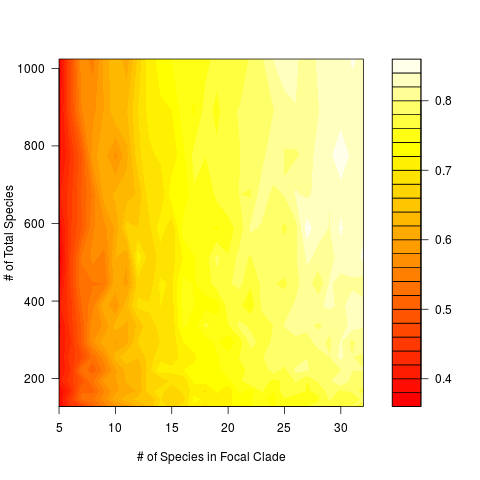
\includegraphics[width=.5\textwidth]{errorRate50.png}
  \caption{\textbf{Mean error rate in the ranking of top 50 species.}}
\end{figure}

\begin{figure}[!ht]
  \center
  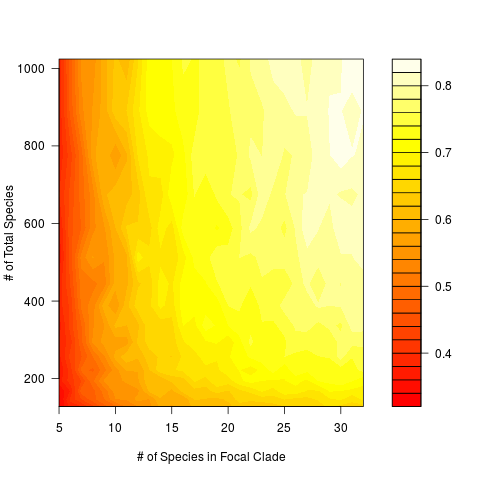
\includegraphics[width=.5\textwidth]{errorRate100.png}
  \caption{\textbf{Mean error rate in the ranking of top 100 species.} }
\end{figure}

\begin{figure}[!ht]
  \center
  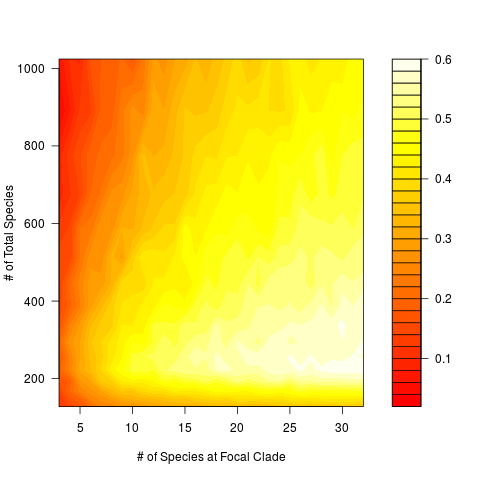
\includegraphics[width=.5\textwidth]{errorRate200.png}
  \caption{\textbf{Mean error rate in the ranking of top 200 species.} }
\end{figure}

\begin{figure}[!ht]
  \center
  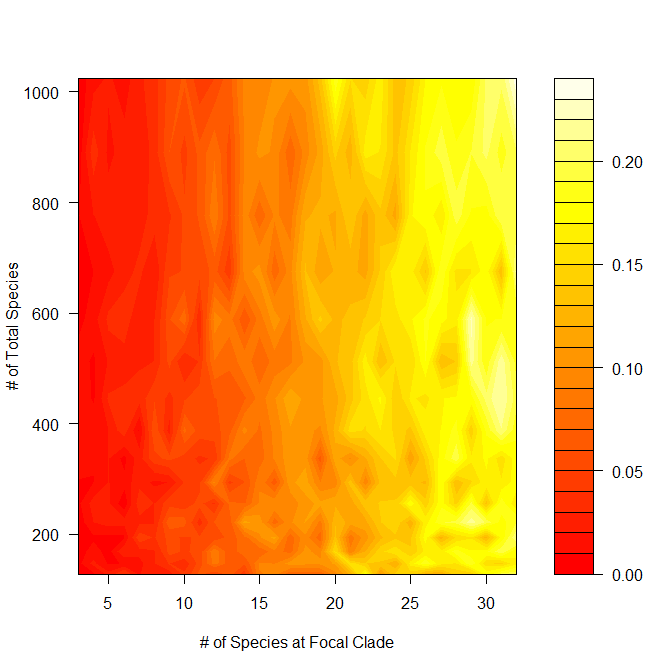
\includegraphics[width=.5\textwidth]{errorRate5pct.png}
  \caption{\textbf{Mean error rate in the ranking of top 5\% of species.} }
\end{figure}

\begin{figure}[!ht]
  \center
  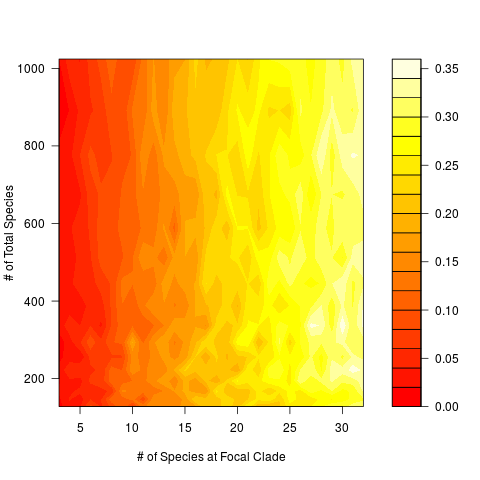
\includegraphics[width=.5\textwidth]{errorRate10pct.png}
  \caption{\textbf{Mean error rate in the ranking of top 10\% of species.} }
\end{figure}

\begin{figure}[!ht]
  \center
  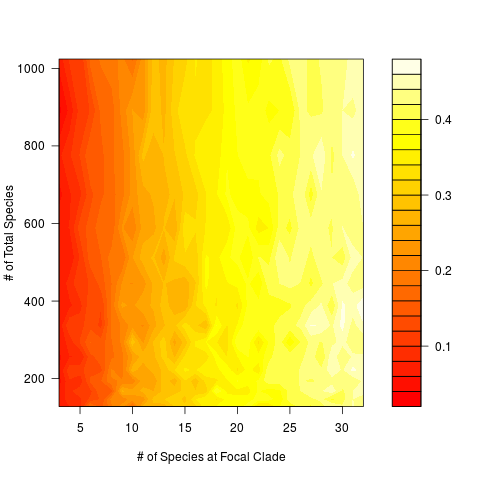
\includegraphics[width=.5\textwidth]{errorRate20pct.png}
  \caption{\textbf{Mean error rate in the ranking of top 20\% of species.}}
\end{figure}

\end{document}
%%% Local Variables:
%%% mode: latex
%%% TeX-master: t
%%% End:
